\section*{Desarrollo}
En esta secci\'on se podran observar los pasos para el diseño del filtro y el detalle de los c\'alculos emplados para lograr la salida requerida, junto con las prubeas y respuestas en frecuencia pedidas.\\

\subsection*{Problema a resolver}
El filtro a diseñar vino dado por la siguiente imagen de un diagrama de \textit{Bode}. \\
\begin{figure}[H]
	\centering
	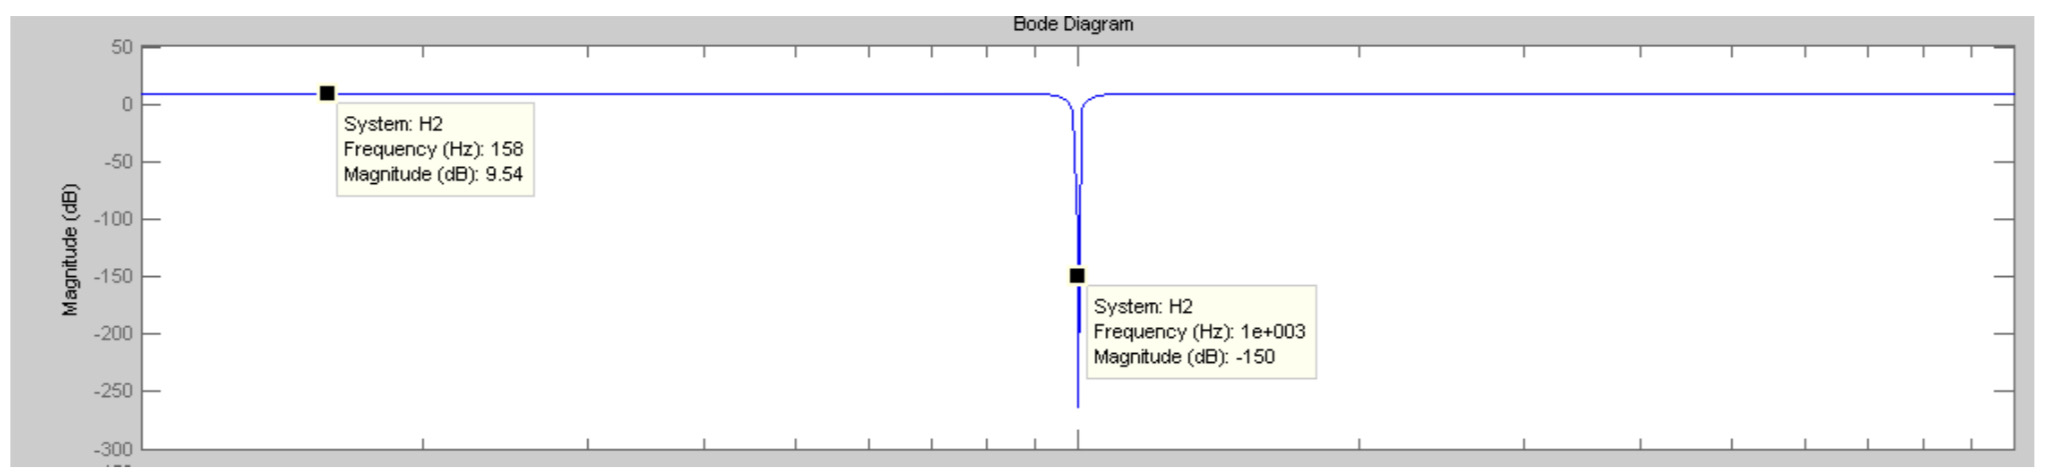
\includegraphics[width=15cm]{imagenes/consigna}
	\caption{Consigna del filtro a diseñar}
	\label{img:consigna}
\end{figure}

Se observa que es un filtro del tipo \textit{Notch} o \textit{Elimina banda} para la frecuencia de $1\kHz$ y tambien que para el resto de las frecuencias, posee un nivel de amplifiaci\'on de $9.54\dB$.

\subsection*{Diseño del filtro}
Se identificaron los par\'ametros de la transferencia del filtro a partir de la forma de Bode vista en clase.\\

\begin{equation}
  H(s)=H_0\ \frac{s^2 + \omega_0 ^2}{s^2 +s \frac{\omega_0}{Q} +\omega_0}
\end{equation}
De la  consigna se ve que la frecuencia de corte es $f_0 = 1\kHz$, por lo que $\omega_0 = 2\pi f_0= 2000\pi$. En $\omega_0$ se encuentra el polo doble de la transferencia.
Luego se eligi\'o un coeficiente de selectividad $Q > \frac{1}{\sqrt 2}$ (para que funcione como elimina banda) pero no tan grande que luego el circuito pueda correr riesgo de comportarse como oscilador. Se eligi\'o $Q= 2.7$ en funci\'on de los valores de resistencia y capacitor convenientes para el circuito.
Luego, del dato del primer punto medido en la consigna, se despej\'o el valor de $H_0$ de la siguiente expresi\'on
\begin{equation}
  H_0^x = 20 \log (H_0^{dB})
\end{equation}
Viendo en la cosigna que los valores de amplificacion fuera de la frecuencia de corte es $9.54 \dB$ se obtiene $H_0 = 3 $.
\subsection*{Circuito}
Se utiliz\'o el siguiente circuito visto en clase
%TODO: insertar circuito  notch sin ampli al final
Aplicando el metodo de \textit{Nodos} se llega a la siguiente transferencia
\begin{equation}
  H(s) = \frac{s^2 \frac{RC}{2}^2+1}{s^2 \frac{RC}{2}^2+s \frac{RC}{2} 4(1-k)+1}
\end{equation}
	Notando que $\omega_0 = \frac{2}{RC}$, se elig\'o  un valor de capacitor tal que la resistencias se encuente entre $1\kohm$ y $1\megohm$. Tambien se consider\'o  que al elegir un valor comercial que diste del valor teorico, va a existir un error. Considerando esto, se eligi\'o $C= 10 \nF$ y $R= 31.6 \kohm$, \'este valor de resistencia es el que menos error presenta del valor teorico ($R_{teo}=31.83 \kohm$).\\
	Hasta ahora, el circuito funciona como elimina banda para la frecuencia de $1\kHz$, pero no amplifica en $9.54 \dB$ el resto de las frecuencias. Para ello, se empleo un amplificador en configuraci\'on \textit{No inverson} a la salida del filtro. Resultando en el siguiente circuito.
%TODO: insertar circuito completo.

\subsection*{Simulaci\'on}
	Para verificar que el funcionamiento del circuito sea el esperado, se utiliz\'o el software de simulaci\'on \textit{LTSpice} con los componentes de valores comerciales. 
\begin{figure}[hbt]
	\centering
	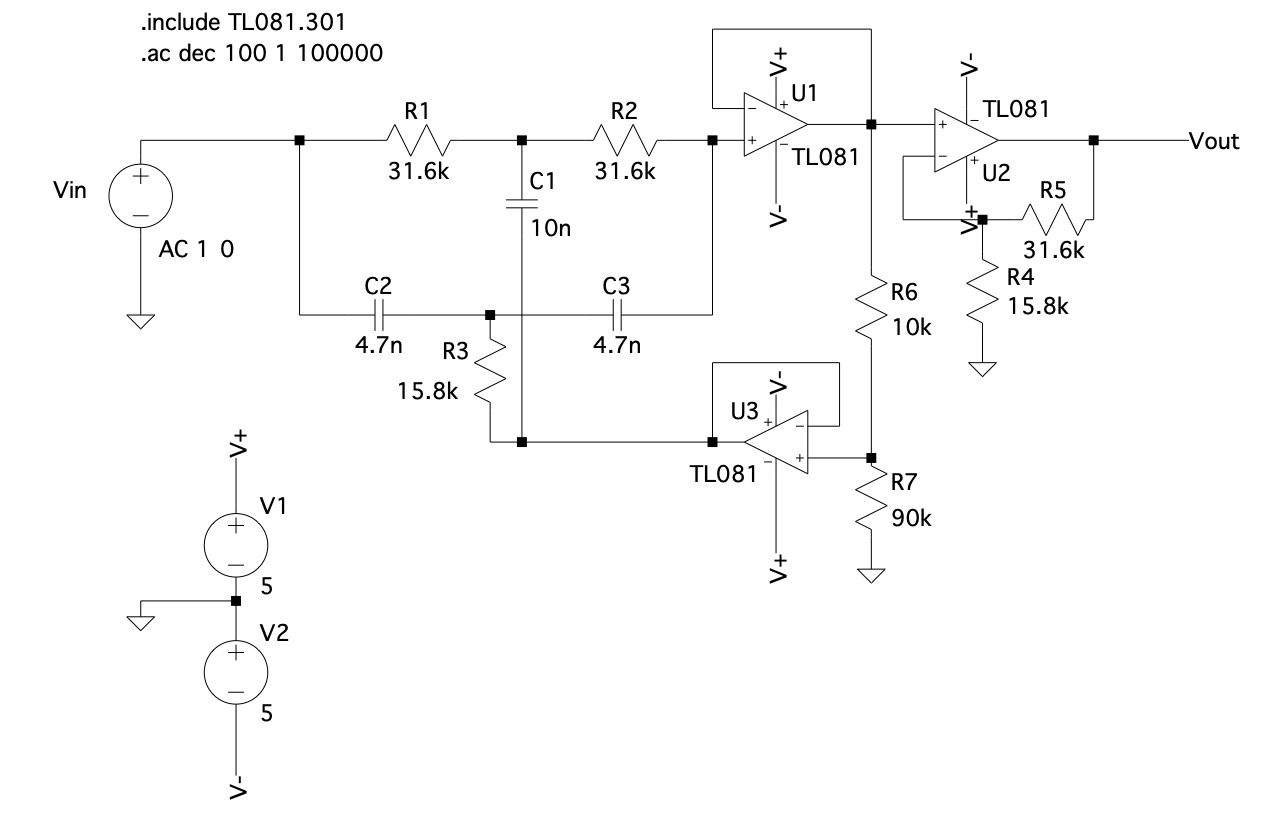
\includegraphics[width=10cm]{imagenes/simulacion}
	\caption{Circtuito simulado}
\end{figure}

	
Se utiliz\'o la directiva \texttt{.ac dec 100 1 1000000 } para
variar la  frecuencia de la fuente de entrada \texttt{ Vin } desde  $1 \si{\hertz}$ hasta $100 \kHz$. Luego se import\'o la biblioteca \textit{TL081} para el operacional. Produciendo el siguiente resultado.

